\section{Capítulo 11 -- Testes e depuração}

Todo programador escreve programas com erros. A diferença entre um iniciante e um profissional não está em errar menos, mas em \textbf{encontrar os erros mais cedo} e \textbf{corrigi-los com método}. Ao longo deste livro, cada capítulo terminou com uma lista de Erros Comuns, e todos os programas foram compilados e executados para conferir as saídas mostradas no texto. Neste último capítulo, você vai aprender a fazer isso de forma sistemática: declarar o que o código espera com \texttt{assert}, escolher bons casos de teste, gerar milhares de testes automaticamente e, quando algo der errado, seguir um roteiro de depuração em vez de mudar o código no escuro.

\subsection{11.1 Tipos de erro}

Os erros de um programa aparecem em três momentos diferentes, e cada um pede uma estratégia:

\begin{center}
\begin{tabular}{@{}p{0.22\linewidth}p{0.36\linewidth}p{0.32\linewidth}@{}}
\toprule
\rowcolor{headergray}
\tblheader{Tipo} & \tblheader{Quando aparece} & \tblheader{Exemplo} \\
\midrule
de compilação & o compilador recusa o programa & ponto e vírgula esquecido, tipo errado, variável não declarada \\
\rowcolor{rowgray} de execução & o programa para no meio & acesso a \texttt{nullptr}, divisão por zero, recursão infinita \\
de lógica & o programa termina, mas a resposta está errada & \texttt{<} no lugar de \texttt{<=}, laço que pula o último elemento \\
\bottomrule
\end{tabular}
\end{center}

Os erros de compilação são os mais fáceis: o compilador diz onde estão. Por isso, vale a pena transformar o máximo de erros possível em erros de compilação, com \texttt{const}, tipos bem escolhidos e os avisos do compilador ligados (\texttt{-Wall -Wextra}). Os erros de lógica são os mais perigosos, porque o programa parece funcionar. São eles que os testes procuram.

\subsection{11.2 Asserções}

Uma \textbf{asserção} é uma condição que o programador garante ser verdadeira em um ponto do código. A \texttt{assert}, da biblioteca \texttt{<cassert>}, verifica a condição durante a execução; se ela for falsa, o programa para na hora, mostrando a condição, o arquivo e a linha. É muito melhor do que continuar com dados errados e falhar muito depois, longe da causa.

As asserções costumam expressar três tipos de garantia:

\begin{itemize}
  \item \textbf{Pré-condição}: o que precisa ser verdade na entrada da função. A busca binária só funciona com o vetor ordenado; a média só faz sentido com pelo menos uma nota.
  \item \textbf{Pós-condição}: o que a função garante na saída. Depois da ordenação, o vetor está ordenado.
  \item \textbf{Invariante}: o que continua verdade durante toda a execução, como ``o tamanho da pilha nunca é negativo'' ou ``a raiz do heap é o maior elemento''.
\end{itemize}

\begin{codigo}
\begin{Verbatim}[breaklines=true, breaksymbolleft={}, fontsize=\footnotesize]
#include <vector>
#include <cassert>
#include <algorithm>   // is_sorted

int buscaBinaria(const vector<int> &v, int procurado) {
    assert(is_sorted(v.begin(), v.end()));   // pré-condição
    int inicio = 0;
    int fim = static_cast<int>(v.size()) - 1;
    while (inicio <= fim) {
        int meio = inicio + (fim - inicio) / 2;
        if (v[meio] == procurado) return meio;
        if (v[meio] < procurado) {
            inicio = meio + 1;
        } else {
            fim = meio - 1;
        }
    }
    return -1;
}

double media(const vector<double> &notas) {
    assert(!notas.empty());                  // pré-condição
    double soma = 0;
    for (double nota : notas) soma += nota;
    return soma / notas.size();
}

int main() {
    cout << buscaBinaria({3, 8, 12, 17}, 12) << endl;   // 2
    cout << media({7.0, 8.0, 9.0}) << endl;             // 8
    // buscaBinaria({8, 3, 12}, 3) pararia o programa com:
    // Assertion failed: is_sorted(v.begin(), v.end()),
    // file busca.cpp, line 6
}
\end{Verbatim}
\end{codigo}

Repare que a asserção da busca binária custa $O(n)$, mais que a própria busca. Asserções servem para encontrar erros durante o desenvolvimento; na versão final, elas podem ser desligadas compilando com a opção \texttt{-DNDEBUG}, e todas as \texttt{assert} desaparecem do programa. Por isso, nunca coloque dentro de uma \texttt{assert} algo que precisa acontecer, como \texttt{assert(pilha.desempilhar() > 0)}: com \texttt{NDEBUG}, a chamada inteira some.

\begin{destaque}{Asserção ou tratamento de erro?}
A \texttt{assert} é para erros do \textbf{programador}: situações que nunca deveriam acontecer se o código estivesse certo. Erros que vêm de \textbf{fora}, como um usuário digitando uma letra onde se esperava um número ou um arquivo que não existe, vão acontecer de verdade e precisam ser tratados pelo programa, com mensagens claras, valores de retorno ou exceções. Um programa não deve parar só porque o usuário errou a digitação.
\end{destaque}

\subsection{11.3 Testes unitários}

Um \textbf{teste unitário} verifica uma pequena parte do programa, normalmente uma função, isoladamente: chama a função com uma entrada conhecida e compara o resultado com o \textbf{valor esperado}, calculado à mão ou por outro meio confiável. É aqui que as funções puras do Capítulo 10 mostram seu valor: como o resultado depende só dos parâmetros, testá-las é só chamar e comparar.

Existem bibliotecas prontas para escrever testes em C++, como a GoogleTest e a Catch2, mas a ideia cabe em poucas linhas. O exemplo testa uma função que classifica a situação de um aluno pela nota:

\begin{codigo}
\begin{Verbatim}[breaklines=true, breaksymbolleft={}, fontsize=\footnotesize]
#include <string>

string situacao(double nota) {
    if (nota < 0 || nota > 10) return "inválida";
    if (nota < 4) return "reprovado";
    if (nota < 6) return "prova final";
    return "aprovado";
}

int falhas = 0;

void verificar(const string &obtido, const string &esperado,
               const string &caso) {
    if (obtido != esperado) {
        falhas++;
        cout << "FALHOU (" << caso << "): esperado " << esperado
             << ", obtido " << obtido << endl;
    }
}

int main() {
    // um valor típico de cada faixa
    verificar(situacao(2), "reprovado", "nota 2");
    verificar(situacao(5), "prova final", "nota 5");
    verificar(situacao(8), "aprovado", "nota 8");
    // as fronteiras, onde os erros costumam estar
    verificar(situacao(0), "reprovado", "nota 0");
    verificar(situacao(3.9), "reprovado", "nota 3,9");
    verificar(situacao(4), "prova final", "nota 4");
    verificar(situacao(5.9), "prova final", "nota 5,9");
    verificar(situacao(6), "aprovado", "nota 6");
    verificar(situacao(10), "aprovado", "nota 10");
    // fora do domínio
    verificar(situacao(-0.1), "inválida", "nota -0,1");
    verificar(situacao(10.1), "inválida", "nota 10,1");

    if (falhas == 0) cout << "11 testes passaram" << endl;
}
\end{Verbatim}
\end{codigo}

Se alguém trocar \texttt{nota < 4} por \texttt{nota <= 4}, o programa continua compilando e parece funcionar com notas como 2 e 8. Mas o teste da nota 4 avisa na hora: \texttt{FALHOU (nota 4): esperado prova final, obtido reprovado}.

\subsubsection{Como escolher os casos}

Testar todas as entradas possíveis é impossível, então os casos precisam ser escolhidos com cuidado. Duas ideias ajudam muito:

\begin{itemize}
  \item \textbf{Faixas de valores} (partições de equivalência): divida as entradas em grupos que o programa deve tratar do mesmo jeito e teste um valor típico de cada grupo. Se a nota 2 funciona, a nota 2,5 quase certamente também funciona.
  \item \textbf{Valores de fronteira}: os erros se concentram nas bordas entre as faixas, onde um \texttt{<} pode estar no lugar de um \texttt{<=}. Teste os valores exatamente nas fronteiras e logo ao lado delas.
\end{itemize}

\begin{center}
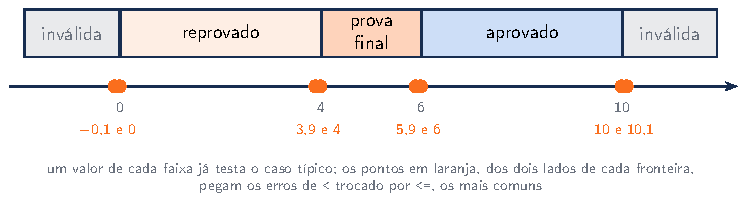
\includegraphics[width=0.95\linewidth,keepaspectratio]{imagens/capitulo-11_fronteiras.pdf}
\end{center}

Para as estruturas de dados deste livro, os casos de fronteira têm uma cara conhecida. Vale a pena testar sempre:

\begin{center}
\begin{tabular}{@{}p{0.3\linewidth}p{0.6\linewidth}@{}}
\toprule
\rowcolor{headergray}
\tblheader{Situação} & \tblheader{Exemplos} \\
\midrule
estrutura vazia & vetor sem elementos, lista com \texttt{inicio == nullptr}, pilha vazia \\
\rowcolor{rowgray} um único elemento & o primeiro é também o último; a raiz não tem filhos \\
primeiro e último & inserir ou remover no início e no fim da lista \\
\rowcolor{rowgray} valor ausente & procurar algo menor que todos, maior que todos, ou entre dois \\
valores repetidos & a busca e a ordenação continuam corretas? A ordenação é estável? \\
\rowcolor{rowgray} entradas já organizadas & vetor já ordenado ou em ordem inversa (o pior caso do \textit{quicksort}) \\
\bottomrule
\end{tabular}
\end{center}

Quando muitos casos seguem o mesmo formato, é prático escrevê-los como uma \textbf{tabela de casos}, um vetor em que cada linha tem a entrada e o que se espera, e testá-los todos com um único laço. O programa abaixo testa a busca binária assim. Em vez de comparar com uma posição exata, ele verifica uma \textbf{propriedade}: se o valor está no vetor, a posição devolvida precisa conter o valor; se não está, o resultado precisa ser $-1$. Isso funciona até com valores repetidos, em que mais de uma posição seria correta.

\begin{codigo}
\begin{Verbatim}[breaklines=true, breaksymbolleft={}, fontsize=\footnotesize]
#include <vector>
#include <string>

int buscaBinaria(const vector<int> &v, int procurado) {
    int inicio = 0;
    int fim = static_cast<int>(v.size()) - 1;
    while (inicio <= fim) {
        int meio = inicio + (fim - inicio) / 2;
        if (v[meio] == procurado) return meio;
        if (v[meio] < procurado) {
            inicio = meio + 1;
        } else {
            fim = meio - 1;
        }
    }
    return -1;
}

struct Caso {
    string descricao;
    vector<int> v;
    int procurado;
    bool presente;
};

int main() {
    const vector<Caso> casos = {
        {"vetor vazio", {}, 5, false},
        {"um elemento, presente", {5}, 5, true},
        {"um elemento, ausente", {5}, 3, false},
        {"primeiro", {2, 4, 6, 8}, 2, true},
        {"último", {2, 4, 6, 8}, 8, true},
        {"menor que todos", {2, 4, 6, 8}, 1, false},
        {"maior que todos", {2, 4, 6, 8}, 9, false},
        {"entre dois", {2, 4, 6, 8}, 5, false},
        {"repetidos", {3, 3, 3, 3, 3}, 3, true},
    };
    int falhas = 0;
    for (const Caso &c : casos) {
        int r = buscaBinaria(c.v, c.procurado);
        bool certo = c.presente
            ? (r >= 0 && c.v[r] == c.procurado)
            : (r == -1);
        if (!certo) {
            falhas++;
            cout << "FALHOU: " << c.descricao << endl;
        }
    }
    cout << casos.size() - falhas << " de " << casos.size()
         << " casos passaram" << endl;   // 9 de 9 casos passaram
}
\end{Verbatim}
\end{codigo}

Acrescentar um caso novo é acrescentar uma linha na tabela. E, sempre que um erro for encontrado, o caso que o revelou deve virar uma linha nova: assim, se o erro voltar algum dia, o teste avisa. Esse é o \textbf{teste de regressão}.

\subsection{11.4 Testes com dados gerados}

Por melhor que seja a escolha dos casos, é fácil esquecer uma combinação. Uma técnica poderosa é \textbf{gerar} milhares de entradas automaticamente e comparar o resultado da sua função com o de um \textbf{oráculo}: outra forma de calcular a mesma resposta que você confia que está certa, mesmo que seja lenta. Para uma função de ordenação, o oráculo natural é a \texttt{sort} da biblioteca padrão.

O programa abaixo testa uma ordenação por inserção (Capítulo 8) que tem um erro escondido: o laço interno usa \texttt{j > 0} em vez de \texttt{j >= 0}. Os vetores são gerados com o \texttt{mt19937}, um gerador de números pseudoaleatórios da biblioteca \texttt{<random>}. Ele recebe uma \textbf{semente} fixa, para que a sequência gerada seja sempre a mesma e uma falha encontrada possa ser repetida.

\begin{codigo}
\begin{Verbatim}[breaklines=true, breaksymbolleft={}, fontsize=\footnotesize]
#include <vector>
#include <random>      // mt19937
#include <algorithm>   // sort

void insercaoComErro(vector<int> &v) {
    for (int i = 1; i < static_cast<int>(v.size()); i++) {
        int chave = v[i];
        int j = i - 1;
        while (j > 0 && v[j] > chave) {   // erro: certo é j >= 0
            v[j + 1] = v[j];
            j--;
        }
        v[j + 1] = chave;
    }
}

void mostrar(const vector<int> &v) {
    for (int x : v) cout << x << " ";
    cout << endl;
}

int main() {
    mt19937 gerador(2026);              // semente fixa: repetível
    for (int teste = 1; teste <= 1000; teste++) {
        int n = gerador() % 6;          // vetores pequenos: 0 a 5
        vector<int> v(n);
        for (int &x : v) x = gerador() % 10;

        vector<int> esperado = v, obtido = v;
        sort(esperado.begin(), esperado.end());   // o oráculo
        insercaoComErro(obtido);
        if (obtido != esperado) {
            cout << "teste " << teste << " falhou com: ";
            mostrar(v);
            cout << "obtido: ";
            mostrar(obtido);
            return 0;
        }
    }
    cout << "1000 testes passaram" << endl;
}
\end{Verbatim}
\end{codigo}

Com a semente 2026, o erro aparece logo no segundo vetor gerado. A saída é:

\begin{center}
\texttt{teste 2 falhou com: 7 7 0} \\
\texttt{obtido: 7 0 7}
\end{center}

O 0 deveria ter ido para o início do vetor, mas parou na posição 1. Com 1.000 vetores testados em uma fração de segundo, um erro que escaparia de muitos testes escritos à mão é encontrado quase de imediato.

Três decisões tornam esse tipo de teste eficiente. Os vetores são \textbf{pequenos} (até 5 elementos), porque quase todo erro já aparece com poucos dados, e um caso pequeno é muito mais fácil de entender. Os valores vêm de uma \textbf{faixa estreita} (0 a 9), para que repetições apareçam com frequência. E a \textbf{semente é fixa}, para que a mesma falha apareça de novo depois de cada tentativa de correção.

Quando um teste gerado falha, o próximo passo é \textbf{reduzir o caso}: apagar elementos um a um enquanto a falha continuar acontecendo. Aqui, apagando um dos 7, chega-se a \texttt{\{7, 0\}}, um vetor de só dois elementos que já mostra o problema: com \texttt{j > 0}, o laço nunca compara com a posição 0, então nenhum elemento consegue chegar ao início do vetor. Corrigido o erro, o caso \texttt{\{7, 0\}} vira mais uma linha da tabela de testes.

\subsection{11.5 Depuração}

Quando um teste falha, começa a \textbf{depuração}: encontrar a causa do erro e corrigi-la. A tentação é sair mudando o código até o resultado parecer certo, mas isso costuma esconder o erro em vez de corrigi-lo. O caminho mais rápido é tratar a depuração como uma investigação, com um passo de cada vez:

\begin{center}
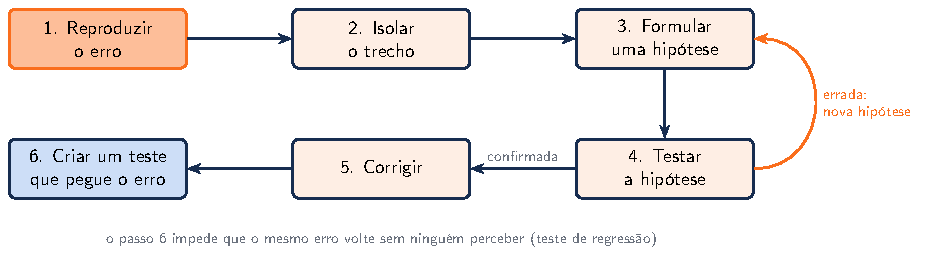
\includegraphics[width=\linewidth,keepaspectratio]{imagens/capitulo-11_ciclo.pdf}
\end{center}

\begin{enumerate}
  \item \textbf{Reproduzir}: encontre uma entrada que sempre faça o erro aparecer. Um erro que não se repete não pode ser investigado nem ter a correção confirmada.
  \item \textbf{Isolar}: reduza a entrada e o código até o menor trecho que ainda mostra o erro. Se a função funciona com a entrada reduzida, o erro está em outro lugar.
  \item \textbf{Formular uma hipótese}: ``acho que o \texttt{meio} está saindo do vetor quando ele tem um só elemento''. Uma hipótese boa é específica e pode ser testada.
  \item \textbf{Testar a hipótese}: mostre os valores das variáveis ou use o depurador para confirmá-la ou descartá-la. Se for descartada, formule outra.
  \item \textbf{Corrigir} a causa, e não o sintoma. Somar 1 ao resultado para ``acertar'' a saída não é uma correção.
  \item \textbf{Criar um teste} com o caso que revelou o erro, para ele não voltar.
\end{enumerate}

\subsubsection{Mostrando o estado do programa}

A técnica mais simples para testar uma hipótese é imprimir os valores das variáveis nos pontos importantes. Use o \texttt{cerr}, a saída de erros, e não o \texttt{cout}: as mensagens de depuração não se misturam com a saída normal do programa e aparecem na hora, mesmo que o programa trave logo depois. Uma constante permite ligar e desligar todas as mensagens de uma vez.

\begin{codigo}
\begin{Verbatim}[breaklines=true, breaksymbolleft={}, fontsize=\footnotesize]
#include <vector>

const bool DEPURAR = true;    // false para desligar as mensagens

int buscaBinaria(const vector<int> &v, int procurado) {
    int inicio = 0;
    int fim = static_cast<int>(v.size()) - 1;
    while (inicio <= fim) {
        int meio = inicio + (fim - inicio) / 2;
        if (DEPURAR) {
            cerr << "inicio=" << inicio << " fim=" << fim
                 << " meio=" << meio << " v[meio]=" << v[meio]
                 << endl;
        }
        if (v[meio] == procurado) return meio;
        if (v[meio] < procurado) {
            inicio = meio + 1;
        } else {
            fim = meio - 1;
        }
    }
    return -1;
}

int main() {
    vector<int> v = {3, 8, 12, 17, 21, 25, 30, 34, 39, 42,
                     47, 51, 56, 60, 64};
    cout << buscaBinaria(v, 20) << endl;
    // na saída de erros:
    // inicio=0 fim=14 meio=7 v[meio]=34
    // inicio=0 fim=6 meio=3 v[meio]=17
    // inicio=4 fim=6 meio=5 v[meio]=25
    // inicio=4 fim=4 meio=4 v[meio]=21
    // e na saída normal: -1
}
\end{Verbatim}
\end{codigo}

As mensagens reproduzem exatamente a tabela da busca pelo 20 no Capítulo 7. Se uma das linhas mostrasse \texttt{inicio} e \texttt{fim} repetindo os mesmos valores, a hipótese de um laço infinito estaria confirmada.

\subsubsection{O depurador}

Um \textbf{depurador} permite pausar o programa em qualquer linha e examinar tudo, sem acrescentar \texttt{cerr} nenhum. O depurador do GCC é o \texttt{gdb}, e as IDEs, como o VS Code, oferecem os mesmos recursos com botões e atalhos. Para usá-lo, compile com a opção \texttt{-g}, que guarda no executável as informações sobre as linhas e os nomes das variáveis.

\begin{center}
\begin{tabular}{@{}p{0.3\linewidth}p{0.2\linewidth}p{0.4\linewidth}@{}}
\toprule
\rowcolor{headergray}
\tblheader{Recurso} & \tblheader{No gdb} & \tblheader{O que faz} \\
\midrule
ponto de parada & \texttt{break 12} & pausa o programa ao chegar na linha 12 (F9 no VS Code) \\
\rowcolor{rowgray} executar & \texttt{run} & inicia o programa, que roda até um ponto de parada \\
próxima linha & \texttt{next} & executa a linha atual sem entrar nas funções chamadas (F10) \\
\rowcolor{rowgray} entrar na função & \texttt{step} & entra na função chamada na linha atual (F11) \\
mostrar valor & \texttt{print meio} & mostra o valor de uma variável ou expressão \\
\rowcolor{rowgray} pilha de chamadas & \texttt{backtrace} & mostra quais funções chamaram quais até aqui \\
vigiar variável & \texttt{watch fim} & pausa sempre que \texttt{fim} mudar de valor \\
\rowcolor{rowgray} continuar & \texttt{continue} & segue até o próximo ponto de parada (F5) \\
\bottomrule
\end{tabular}
\end{center}

A pilha de chamadas é especialmente útil quando o programa para com um erro de execução: ela mostra a linha exata do problema e todo o caminho de chamadas até ele. Em uma recursão infinita, por exemplo, aparece a mesma função repetida milhares de vezes.

\begin{destaque}{Outras ferramentas que encontram erros sozinhas}
\begin{itemize}
  \item \textbf{Avisos do compilador}: \texttt{-Wall -Wextra} apontam variáveis não usadas, comparações suspeitas e funções que podem terminar sem \texttt{return}. Trate cada aviso como um erro.
  \item \textbf{Sanitizadores}: são verificações extras que o compilador acrescenta ao programa. Elas fazem o programa parar e explicar o problema ao ler fora de um vetor, usar memória depois do \texttt{delete} ou estourar um \texttt{int}, erros que normalmente passariam em silêncio. No Linux e no macOS, são ligadas com as opções \texttt{-fsanitize=address} e \texttt{-fsanitize=undefined}.
  \item \textbf{Busca binária no histórico}: se o programa funcionava em uma versão antiga e não funciona mais, o comando \texttt{git bisect} faz uma busca binária (Capítulo 7) nas versões salvas e encontra a mudança que introduziu o erro testando só $\log_2 n$ delas.
  \item \textbf{Explicar em voz alta}: descrever o código linha por linha para outra pessoa, ou até para um patinho de borracha na mesa, obriga a olhar para o que o código faz, e não para o que se acha que ele faz. É surpreendente quantos erros aparecem no meio da explicação.
\end{itemize}
\end{destaque}

\subsection{11.6 Sintomas e causas prováveis}

Com o tempo, cada sintoma passa a sugerir algumas causas. Esta tabela reúne as mais comuns nas estruturas deste livro:

\begin{center}
\begin{tabular}{@{}p{0.34\linewidth}p{0.56\linewidth}@{}}
\toprule
\rowcolor{headergray}
\tblheader{Sintoma} & \tblheader{Causas prováveis} \\
\midrule
o programa trava e não termina & laço cuja condição nunca muda, como a busca binária com \texttt{inicio = meio} (Capítulo 7) \\
\rowcolor{rowgray} o programa fecha sem mensagem & ponteiro \texttt{nullptr} desreferenciado (Capítulos 3 a 5); índice fora do vetor \\
erro de pilha (\textit{stack overflow}) & recursão sem caso base, ou funda demais, como o \textit{quicksort} com vetor ordenado (Capítulo 8) \\
\rowcolor{rowgray} resposta errada só em alguns casos & erro de fronteira: \texttt{<} no lugar de \texttt{<=}, laço que começa ou termina uma posição antes \\
número negativo ou absurdo & estouro de \texttt{int}, como em \texttt{inicio + fim} ou no Fibonacci (Capítulos 7 e 9) \\
\rowcolor{rowgray} resultado muda a cada execução & variável não inicializada; leitura fora do vetor; memória usada depois do \texttt{delete} \\
memória cresce sem parar & \texttt{new} sem o \texttt{delete} correspondente (Capítulo 1) \\
\rowcolor{rowgray} casas decimais somem & divisão entre inteiros; \texttt{accumulate} começando em \texttt{0} em vez de \texttt{0.0} (Capítulo 10) \\
\bottomrule
\end{tabular}
\end{center}

\begin{destaque}{Comparando com Python}
Em Python, \texttt{assert} é um comando da linguagem, e o módulo \texttt{unittest}, que já vem instalado, organiza os testes em classes: cada método que começa com \texttt{test} é um teste, e os métodos \texttt{assertEqual}, \texttt{assertTrue} e semelhantes comparam o obtido com o esperado. Muitos projetos usam a biblioteca externa \texttt{pytest}, ainda mais simples, e a \texttt{hypothesis}, que gera dados de teste e reduz os casos que falham automaticamente.

\begin{codigo}
\begin{Verbatim}[breaklines=true, breaksymbolleft={}, fontsize=\footnotesize]
import random
import unittest

def situacao(nota):
    if nota < 0 or nota > 10:
        return 'inválida'
    if nota < 4:
        return 'reprovado'
    if nota < 6:
        return 'prova final'
    return 'aprovado'

class TestaSituacao(unittest.TestCase):
    def test_fronteiras(self):
        self.assertEqual(situacao(4), 'prova final')
        self.assertEqual(situacao(6), 'aprovado')
        self.assertEqual(situacao(10), 'aprovado')

    def test_invalidas(self):
        self.assertEqual(situacao(-0.1), 'inválida')
        self.assertEqual(situacao(10.1), 'inválida')

    def test_dados_gerados(self):
        random.seed(2026)                   # semente fixa
        for _ in range(1000):
            nota = random.uniform(0, 10)
            self.assertNotEqual(situacao(nota), 'inválida')

unittest.main(argv=['testes'], exit=False)   # Ran 3 tests ... OK
\end{Verbatim}
\end{codigo}

Para depurar, o Python tem o \texttt{pdb}: basta escrever \texttt{breakpoint()} em qualquer linha, e o programa pausa ali, aceitando comandos parecidos com os do \texttt{gdb}, como \texttt{n} (próxima linha), \texttt{s} (entrar na função) e \texttt{p} (mostrar um valor).
\end{destaque}

\subsection{Erros Comuns}

\begin{itemize}
  \item \textbf{Testar só o caso feliz.} Um teste com a nota 8 não pega o erro da nota 4. Teste as fronteiras e as entradas vazias.
  \item \textbf{Calcular o valor esperado com o próprio código testado.} Se a função tem um erro, o ``esperado'' terá o mesmo erro. Use contas feitas à mão ou um oráculo independente.
  \item \textbf{Usar uma semente diferente a cada execução nos testes gerados.} Uma falha que não se repete não pode ser investigada. Fixe a semente, ou pelo menos mostre qual foi usada.
  \item \textbf{Colocar efeitos dentro de \texttt{assert}.} Com \texttt{-DNDEBUG}, a expressão inteira desaparece, junto com o que ela fazia.
  \item \textbf{Usar \texttt{assert} para erros do usuário.} Entradas inválidas precisam de tratamento, não de um programa que para.
  \item \textbf{Mudar o código ao acaso até o teste passar.} Sem entender a causa, a ``correção'' costuma esconder o erro ou criar outro.
  \item \textbf{Ignorar os avisos do compilador.} Muitos erros de lógica aparecem primeiro como um aviso que ninguém leu.
  \item \textbf{Esquecer o teste de regressão.} Todo erro corrigido deve deixar um teste para trás.
\end{itemize}

\subsection{Para continuar}

Este capítulo fecha a parte principal do livro; os Apêndices A e B, a seguir, tratam de tabelas hash e de arquivos. Você começou com ponteiros e memória dinâmica, construiu listas, pilhas, filas, árvores, grafos e heaps, aprendeu a medir o custo de cada algoritmo, a buscar, a ordenar, a otimizar com algoritmos gulosos e programação dinâmica, a escrever no estilo funcional e, por fim, a testar e depurar. As mesmas ideias aparecem em qualquer linguagem e em qualquer sistema grande, de um banco de dados ao mapa do celular. O próximo passo é praticar: implemente as estruturas sem olhar o livro, resolva problemas em sites de programação competitiva e leia o código de bibliotecas que você usa. Bons estudos.
